\subsection{Person 2 – SUS SUS 85{,}0}
\textbf{Zur Person:}\\
Architektin, 62 Jahre alt\\

\textbf{Beobachtung:}
\begin{enumerate}
    \item Zeichnen Sie frei für etwa 2 Minuten.
    \begin{itemize}
        \item Nach dem Ansetzen des Stifts dauerte es einen kurzen Moment, bis das System reagierte, wodurch der Punkt nicht exakt dort erschien, wo sich die Stiftspitze befand.
        \item Geschwindigkeit beeinträchtigte die Genauigkeit.
        \item Insgesamt gutes Feedback, insbesondere wenn dem System etwas Zeit gegeben wird.
    \end{itemize}

    \item Löschen Sie Ihre Zeichnung vollständig.
    \begin{itemize}
        \item Keine Probleme.
    \end{itemize}

    \item Laden Sie die PDF-Datei mit dem Grundriss \texttt{Hospital\_Floor\_Plan.pdf} hoch.
    \begin{itemize}
        \item Kein Problem beim Hochladen.
        \item Kommentar: Bedienung erfordert CAD-Erfahrung. Der verwendete Button war das einzige Symbol, das selbsterklärend wirkte.
        \item Nicht selbstverständlich für unerfahrene Nutzer:innen.
        \item Nachfrage der Testperson: «Kann ich jetzt Wände verschieben?»
    \end{itemize}

    \item Ändern Sie die Stiftfarbe auf Rot.
    \begin{itemize}
        \item Kommentar: «Gut kann ich Englisch.»
    \end{itemize}

    \item Suchen Sie \texttt{BEDROOM3} und zeichnen Sie einen Tisch links vom Bett.
    \begin{itemize}
        \item Keine Probleme.
    \end{itemize}

    \item Radieren Sie den Tisch und zeichnen Sie ihn rechts vom Bett.
    \begin{itemize}
        \item Reaktion: Am falschen Ort schreiben funktioniert nicht.
    \end{itemize}

    \item Zeichnen Sie die Abmessungen 1\,m $\times$ 1\,m und schreiben Sie «table» hinein.
    \begin{itemize}
        \item Keine Probleme.
    \end{itemize}

    \item Speichern Sie den Plan auf Ihrem Laptop.
    \begin{itemize}
        \item Keine Probleme.
    \end{itemize}
\end{enumerate}

\clearpage

\textbf{SUS-Antworten (Bild):}
\begin{center}
    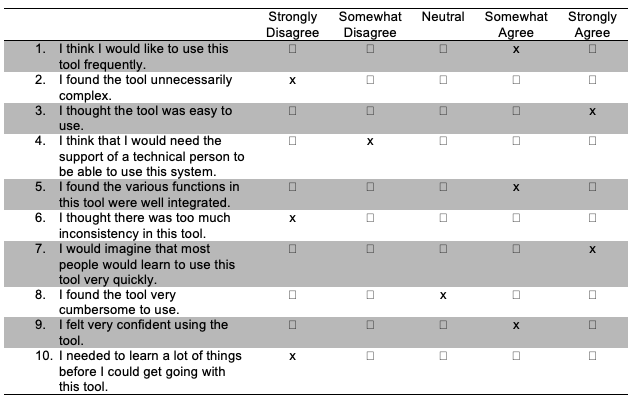
\includegraphics[width=0.95\textwidth]{graphics/sus_person2.png}
\end{center}

\textbf{Follow-up:}
\begin{enumerate}
    \item \textbf{Was hat Ihnen am Tool am besten gefallen?}
    \begin{itemize}
        \item Einfaches Umschalten zwischen Funktionen.
        \item Radiergummi funktioniert gut; Wunsch: einzelne Striche gezielt löschen können.
    \end{itemize}

    \item \textbf{Gab es etwas, das verwirrend oder schwierig zu bedienen war?}
    \begin{itemize}
        \item Nein.
        \item Kommentar: Funktion zum einfachen Wechseln zwischen Plänen und Dokumenten wurde nicht ausprobiert; als Architekt wäre dies wünschenswert.
    \end{itemize}

    \item \textbf{Fehlt etwas, das Sie erwartet oder gerne gehabt hätten?}
    \begin{itemize}
        \item Nein.
    \end{itemize}

    \item \textbf{Haben Sie Vorschläge, wie das Tool verbessert werden könnte?}
    \begin{itemize}
        \item Verschiedene Pläne überlagern.
        \item Wechsel zwischen Plänen ohne vorheriges Speichern ermöglichen.
    \end{itemize}
\end{enumerate}

\clearpage
